\documentclass[twoside]{book}

% Packages required by doxygen
\usepackage{fixltx2e}
\usepackage{calc}
\usepackage{doxygen}
\usepackage[export]{adjustbox} % also loads graphicx
\usepackage{graphicx}
\usepackage[utf8]{inputenc}
\usepackage{makeidx}
\usepackage{multicol}
\usepackage{multirow}
\PassOptionsToPackage{warn}{textcomp}
\usepackage{textcomp}
\usepackage[nointegrals]{wasysym}
\usepackage[table]{xcolor}

% NLS support packages
\usepackage[spanish]{babel}
% Font selection
\usepackage[T1]{fontenc}
\usepackage[scaled=.90]{helvet}
\usepackage{courier}
\usepackage{amssymb}
\usepackage{sectsty}
\renewcommand{\familydefault}{\sfdefault}
\allsectionsfont{%
  \fontseries{bc}\selectfont%
  \color{darkgray}%
}
\renewcommand{\DoxyLabelFont}{%
  \fontseries{bc}\selectfont%
  \color{darkgray}%
}
\newcommand{\+}{\discretionary{\mbox{\scriptsize$\hookleftarrow$}}{}{}}

% Page & text layout
\usepackage{geometry}
\geometry{%
  a4paper,%
  top=2.5cm,%
  bottom=2.5cm,%
  left=2.5cm,%
  right=2.5cm%
}
\tolerance=750
\hfuzz=15pt
\hbadness=750
\setlength{\emergencystretch}{15pt}
\setlength{\parindent}{0cm}
\setlength{\parskip}{3ex plus 2ex minus 2ex}
\makeatletter
\renewcommand{\paragraph}{%
  \@startsection{paragraph}{4}{0ex}{-1.0ex}{1.0ex}{%
    \normalfont\normalsize\bfseries\SS@parafont%
  }%
}
\renewcommand{\subparagraph}{%
  \@startsection{subparagraph}{5}{0ex}{-1.0ex}{1.0ex}{%
    \normalfont\normalsize\bfseries\SS@subparafont%
  }%
}
\makeatother

% Headers & footers
\usepackage{fancyhdr}
\pagestyle{fancyplain}
\fancyhead[LE]{\fancyplain{}{\bfseries\thepage}}
\fancyhead[CE]{\fancyplain{}{}}
\fancyhead[RE]{\fancyplain{}{\bfseries\leftmark}}
\fancyhead[LO]{\fancyplain{}{\bfseries\rightmark}}
\fancyhead[CO]{\fancyplain{}{}}
\fancyhead[RO]{\fancyplain{}{\bfseries\thepage}}
\fancyfoot[LE]{\fancyplain{}{}}
\fancyfoot[CE]{\fancyplain{}{}}
\fancyfoot[RE]{\fancyplain{}{\bfseries\scriptsize Generado por Doxygen }}
\fancyfoot[LO]{\fancyplain{}{\bfseries\scriptsize Generado por Doxygen }}
\fancyfoot[CO]{\fancyplain{}{}}
\fancyfoot[RO]{\fancyplain{}{}}
\renewcommand{\footrulewidth}{0.4pt}
\renewcommand{\chaptermark}[1]{%
  \markboth{#1}{}%
}
\renewcommand{\sectionmark}[1]{%
  \markright{\thesection\ #1}%
}

% Indices & bibliography
\usepackage{natbib}
\usepackage[titles]{tocloft}
\setcounter{tocdepth}{3}
\setcounter{secnumdepth}{5}
\makeindex

% Hyperlinks (required, but should be loaded last)
\usepackage{ifpdf}
\ifpdf
  \usepackage[pdftex,pagebackref=true]{hyperref}
\else
  \usepackage[ps2pdf,pagebackref=true]{hyperref}
\fi
\hypersetup{%
  colorlinks=true,%
  linkcolor=blue,%
  citecolor=blue,%
  unicode%
}

% Custom commands
\newcommand{\clearemptydoublepage}{%
  \newpage{\pagestyle{empty}\cleardoublepage}%
}

\usepackage{caption}
\captionsetup{labelsep=space,justification=centering,font={bf},singlelinecheck=off,skip=4pt,position=top}

%===== C O N T E N T S =====

\begin{document}

% Titlepage & ToC
\hypersetup{pageanchor=false,
             bookmarksnumbered=true,
             pdfencoding=unicode
            }
\pagenumbering{roman}
\begin{titlepage}
\vspace*{7cm}
\begin{center}%
{\Large Tree\+K\+EA \\[1ex]\large version 29-\/may-\/2018 }\\
\vspace*{1cm}
{\large Generado por Doxygen 1.8.11}\\
\end{center}
\end{titlepage}
\clearemptydoublepage
\tableofcontents
\clearemptydoublepage
\pagenumbering{arabic}
\hypersetup{pageanchor=true}

%--- Begin generated contents ---
\chapter{Tree\+K\+EA}
\label{index}\hypertarget{index}{}En esta práctica se construye un programa modular que ofrece un menú de opciones para gestionar un almacén. Se introducen las clases {\itshape \hyperlink{class_almacen}{Almacen}}, {\itshape \hyperlink{class_sala}{Sala}} y {\itshape \hyperlink{class_sistema}{Sistema}}. 
\chapter{Índice de clases}
\section{Lista de clases}
Lista de las clases, estructuras, uniones e interfaces con una breve descripción\+:\begin{DoxyCompactList}
\item\contentsline{section}{\hyperlink{class_almacen}{Almacen} \\*Representa un almacén }{\pageref{class_almacen}}{}
\item\contentsline{section}{\hyperlink{class_sala}{Sala} \\*Representa una sala }{\pageref{class_sala}}{}
\item\contentsline{section}{\hyperlink{class_sistema}{Sistema} \\*Representa un sistema }{\pageref{class_sistema}}{}
\end{DoxyCompactList}

\chapter{Indice de archivos}
\section{Lista de archivos}
Lista de todos los archivos con descripciones breves\+:\begin{DoxyCompactList}
\item\contentsline{section}{\hyperlink{_almacen_8cc}{Almacen.\+cc} \\*Código de la clase \hyperlink{class_almacen}{Almacen} }{\pageref{_almacen_8cc}}{}
\item\contentsline{section}{\hyperlink{_almacen_8hh}{Almacen.\+hh} \\*Especificación de la clase \hyperlink{class_almacen}{Almacen} }{\pageref{_almacen_8hh}}{}
\item\contentsline{section}{\hyperlink{program_8cc}{program.\+cc} \\*Programa principal para el ejercicio {\itshape Tree\+K\+EA} }{\pageref{program_8cc}}{}
\item\contentsline{section}{\hyperlink{_sala_8cc}{Sala.\+cc} \\*Código de la clase \hyperlink{class_sala}{Sala} }{\pageref{_sala_8cc}}{}
\item\contentsline{section}{\hyperlink{_sala_8hh}{Sala.\+hh} \\*Especificación de la clase \hyperlink{class_sala}{Sala} }{\pageref{_sala_8hh}}{}
\item\contentsline{section}{\hyperlink{_sistema_8cc}{Sistema.\+cc} \\*Código de la clase \hyperlink{class_sistema}{Sistema} }{\pageref{_sistema_8cc}}{}
\item\contentsline{section}{\hyperlink{_sistema_8hh}{Sistema.\+hh} \\*Especificación de la clase \hyperlink{class_sistema}{Sistema} }{\pageref{_sistema_8hh}}{}
\end{DoxyCompactList}

\chapter{Documentación de las clases}
\hypertarget{class_almacen}{}\section{Referencia de la Clase Almacen}
\label{class_almacen}\index{Almacen@{Almacen}}


Representa un almacén.  


\subsection*{Métodos públicos}
\begin{DoxyCompactItemize}
\item 
\hyperlink{class_almacen_a68a6084d5775d391c52d4825072a0612}{Almacen} ()
\begin{DoxyCompactList}\small\item\em Creadora por defecto. \end{DoxyCompactList}\item 
void \hyperlink{class_almacen_ae953db6cd573ea3f54e6a02245a25175}{inicializar} (int n)
\begin{DoxyCompactList}\small\item\em Se inicializa el almacén. \end{DoxyCompactList}\item 
int \hyperlink{class_almacen_a0285105782dc12b843cbdad492887956}{poner\+\_\+items} (int id, string prod, int n, \hyperlink{class_sistema}{Sistema} \&sist)
\begin{DoxyCompactList}\small\item\em Si el producto no existe se produce un error y se devuelve -\/1. Se colocan tantas unidades como quepan en la sala y se devuelve un entero que indique cuántas unidades no han cabido. Se colocarán las unidades lo antes posible, es decir, primero se rellenan los huecos a partir del hueco que vaya antes. Las unidades que no quepan no se guardan en el almacén. \end{DoxyCompactList}\item 
int \hyperlink{class_almacen_a2ed6c0f1a88f8ba8d2ad2268640a890f}{quitar\+\_\+items} (int id, string prod, int n, \hyperlink{class_sistema}{Sistema} \&sist)
\begin{DoxyCompactList}\small\item\em Si el producto no existe se produce un error y se devuelve -\/1. Se quitan tantas unidades como se pueda y se devuelve un entero que indique cuántas unidades no se han podido quitar porque no había suficientes en la sala. Se comenzará quitando las unidades que vayan antes. \end{DoxyCompactList}\item 
int \hyperlink{class_almacen_a257546bb178d1bc7b08443697560281a}{distribuir} (string prod, int n, \hyperlink{class_sistema}{Sistema} \&sist)
\begin{DoxyCompactList}\small\item\em Si el producto no existe se produce un error y se devuelve -\/1. Se distribuye el producto según la política explicada en el enunciado. Se devuelve un entero que indica cuántas unidades no se han podido distribuir. Las unidades que no se distribuyan no se guardan en el almacén. \end{DoxyCompactList}\item 
void \hyperlink{class_almacen_a9b0a893ac5ea4774bd362e297b2c3770}{compactar} (int id)
\begin{DoxyCompactList}\small\item\em Se compacta la estantería de la sala. \end{DoxyCompactList}\item 
void \hyperlink{class_almacen_a9e27219c735096dab9d5d3edc2ae2012}{reorganizar} (int id)
\begin{DoxyCompactList}\small\item\em Se reorganiza la estantería de la sala. \end{DoxyCompactList}\item 
void \hyperlink{class_almacen_a477373756d8671d1acef1c7d84a926a9}{redimensionar} (int id, int f, int c)
\begin{DoxyCompactList}\small\item\em Si los productos que hay en la sala no caben en las nuevas dimensiones se produce un error. En caso contrario se compacta la estantería y pasa a tener las nuevas dimensiones. \end{DoxyCompactList}\item 
\hyperlink{class_sala}{Sala} \hyperlink{class_almacen_ad9a5ab33dd0c247c5d09496fa7d202f1}{consultar\+\_\+sal} (int id) const 
\begin{DoxyCompactList}\small\item\em Se devuelve la sala cuyo identificador es el entero. \end{DoxyCompactList}\end{DoxyCompactItemize}
\subsection*{Métodos privados}
\begin{DoxyCompactItemize}
\item 
int \hyperlink{class_almacen_a43e976815927fb9ce06938889d585937}{i\+\_\+distribuir} (string prod, int n, const Bin\+Tree$<$ int $>$ \&\hyperlink{class_almacen_a0800dd9ff516f710e4cff89b6f5d5a4a}{aid})
\begin{DoxyCompactList}\small\item\em Inmersión de distribuir. \end{DoxyCompactList}\item 
void \hyperlink{class_almacen_a16c293b757e28baf6abb9ba926d70c66}{read\+\_\+bintree\+\_\+int} (Bin\+Tree$<$ int $>$ \&a, int marca)
\begin{DoxyCompactList}\small\item\em Se lee la estructura del almacén en preorden. \end{DoxyCompactList}\end{DoxyCompactItemize}
\subsection*{Atributos privados}
\begin{DoxyCompactItemize}
\item 
Bin\+Tree$<$ int $>$ \hyperlink{class_almacen_a0800dd9ff516f710e4cff89b6f5d5a4a}{aid}
\begin{DoxyCompactList}\small\item\em Árbol de identificadores de sala. \end{DoxyCompactList}\item 
vector$<$ \hyperlink{class_sala}{Sala} $>$ \hyperlink{class_almacen_acae00c6ee986edf2a66b07987896b495}{vsal}
\begin{DoxyCompactList}\small\item\em Vector de salas. \end{DoxyCompactList}\end{DoxyCompactItemize}


\subsection{Descripción detallada}
Representa un almacén. 

Definición en la línea 27 del archivo Almacen.\+hh.



\subsection{Documentación del constructor y destructor}
\index{Almacen@{Almacen}!Almacen@{Almacen}}
\index{Almacen@{Almacen}!Almacen@{Almacen}}
\subsubsection[{\texorpdfstring{Almacen()}{Almacen()}}]{\setlength{\rightskip}{0pt plus 5cm}Almacen\+::\+Almacen (
\begin{DoxyParamCaption}
{}
\end{DoxyParamCaption}
)}\hypertarget{class_almacen_a68a6084d5775d391c52d4825072a0612}{}\label{class_almacen_a68a6084d5775d391c52d4825072a0612}


Creadora por defecto. 

\begin{DoxyPrecond}{Precondición}
{\itshape cierto} 
\end{DoxyPrecond}
\begin{DoxyPostcond}{Postcondición}
El resultado es un almacén. 
\end{DoxyPostcond}


Definición en la línea 29 del archivo Almacen.\+cc.


\begin{DoxyCode}
29                  \{
30 \}
\end{DoxyCode}


\subsection{Documentación de las funciones miembro}
\index{Almacen@{Almacen}!i\+\_\+distribuir@{i\+\_\+distribuir}}
\index{i\+\_\+distribuir@{i\+\_\+distribuir}!Almacen@{Almacen}}
\subsubsection[{\texorpdfstring{i\+\_\+distribuir(string prod, int n, const Bin\+Tree$<$ int $>$ \&aid)}{i_distribuir(string prod, int n, const BinTree< int > &aid)}}]{\setlength{\rightskip}{0pt plus 5cm}int Almacen\+::i\+\_\+distribuir (
\begin{DoxyParamCaption}
\item[{string}]{prod, }
\item[{int}]{n, }
\item[{const Bin\+Tree$<$ int $>$ \&}]{aid}
\end{DoxyParamCaption}
)\hspace{0.3cm}{\ttfamily [private]}}\hypertarget{class_almacen_a43e976815927fb9ce06938889d585937}{}\label{class_almacen_a43e976815927fb9ce06938889d585937}


Inmersión de distribuir. 

\begin{DoxyPrecond}{Precondición}
parámetro implícito inicializado, prod existe, n $>$= 0 
\end{DoxyPrecond}
\begin{DoxyPostcond}{Postcondición}
Se distribuye prod según la política explicada en el enunciado empezando por la sala aid.\+value(). Se devuelve un entero que indica cuántas unidades no se han podido distribuir. Las unidades que no se distribuyan no se guardan en el parámetro implícito. 
\end{DoxyPostcond}


Definición en la línea 9 del archivo Almacen.\+cc.


\begin{DoxyCode}
9                                                                      \{
10     \textcolor{keywordflow}{if} (n == 0 or \hyperlink{class_almacen_a0800dd9ff516f710e4cff89b6f5d5a4a}{aid}.empty()) \textcolor{keywordflow}{return} n;
11     n = \hyperlink{class_almacen_acae00c6ee986edf2a66b07987896b495}{vsal}[\hyperlink{class_almacen_a0800dd9ff516f710e4cff89b6f5d5a4a}{aid}.value() - 1].poner\_items(prod, n);
12     \textcolor{keywordflow}{return} \hyperlink{class_almacen_a43e976815927fb9ce06938889d585937}{i\_distribuir}(prod, n/2 + n%2, \hyperlink{class_almacen_a0800dd9ff516f710e4cff89b6f5d5a4a}{aid}.left()) + 
      \hyperlink{class_almacen_a43e976815927fb9ce06938889d585937}{i\_distribuir}(prod, n/2, \hyperlink{class_almacen_a0800dd9ff516f710e4cff89b6f5d5a4a}{aid}.right());
13 \}
\end{DoxyCode}
\index{Almacen@{Almacen}!read\+\_\+bintree\+\_\+int@{read\+\_\+bintree\+\_\+int}}
\index{read\+\_\+bintree\+\_\+int@{read\+\_\+bintree\+\_\+int}!Almacen@{Almacen}}
\subsubsection[{\texorpdfstring{read\+\_\+bintree\+\_\+int(\+Bin\+Tree$<$ int $>$ \&a, int marca)}{read_bintree_int(BinTree< int > &a, int marca)}}]{\setlength{\rightskip}{0pt plus 5cm}void Almacen\+::read\+\_\+bintree\+\_\+int (
\begin{DoxyParamCaption}
\item[{Bin\+Tree$<$ int $>$ \&}]{a, }
\item[{int}]{marca}
\end{DoxyParamCaption}
)\hspace{0.3cm}{\ttfamily [private]}}\hypertarget{class_almacen_a16c293b757e28baf6abb9ba926d70c66}{}\label{class_almacen_a16c293b757e28baf6abb9ba926d70c66}


Se lee la estructura del almacén en preorden. 

\begin{DoxyPrecond}{Precondición}
a.\+empty() 
\end{DoxyPrecond}
\begin{DoxyPostcond}{Postcondición}
Se lee la estructura del parámetro implícito en preorden. 
\end{DoxyPostcond}


Definición en la línea 16 del archivo Almacen.\+cc.


\begin{DoxyCode}
16                                                          \{
17     \textcolor{keywordtype}{int} x;
18     cin >> x;
19     \textcolor{keywordflow}{if} (x != marca) \{
20         BinTree<int> l;
21         \hyperlink{class_almacen_a16c293b757e28baf6abb9ba926d70c66}{read\_bintree\_int}(l, marca);
22         BinTree<int> r;
23         \hyperlink{class_almacen_a16c293b757e28baf6abb9ba926d70c66}{read\_bintree\_int}(r, marca);
24         a = BinTree<int>(x, l, r);
25     \}
26 \}
\end{DoxyCode}
\index{Almacen@{Almacen}!inicializar@{inicializar}}
\index{inicializar@{inicializar}!Almacen@{Almacen}}
\subsubsection[{\texorpdfstring{inicializar(int n)}{inicializar(int n)}}]{\setlength{\rightskip}{0pt plus 5cm}void Almacen\+::inicializar (
\begin{DoxyParamCaption}
\item[{int}]{n}
\end{DoxyParamCaption}
)}\hypertarget{class_almacen_ae953db6cd573ea3f54e6a02245a25175}{}\label{class_almacen_ae953db6cd573ea3f54e6a02245a25175}


Se inicializa el almacén. 

\begin{DoxyPrecond}{Precondición}
parámetro implícito no inicializado, n $>$ 0 
\end{DoxyPrecond}
\begin{DoxyPostcond}{Postcondición}
Se inicializa el parámetro implícito. 
\end{DoxyPostcond}


Definición en la línea 33 del archivo Almacen.\+cc.


\begin{DoxyCode}
33                                \{
34     \hyperlink{class_almacen_a16c293b757e28baf6abb9ba926d70c66}{read\_bintree\_int}(\hyperlink{class_almacen_a0800dd9ff516f710e4cff89b6f5d5a4a}{aid}, 0);
35     \hyperlink{class_almacen_acae00c6ee986edf2a66b07987896b495}{vsal} = vector<Sala>(n);
36     \textcolor{keywordflow}{for} (\textcolor{keywordtype}{int} i = 0; i < \hyperlink{class_almacen_acae00c6ee986edf2a66b07987896b495}{vsal}.size(); ++i) \{
37         \textcolor{keywordtype}{int} f, c;
38         cin >> f >> c;
39         \hyperlink{class_almacen_acae00c6ee986edf2a66b07987896b495}{vsal}[i].inicializar(f, c);
40     \}
41 \}
\end{DoxyCode}
\index{Almacen@{Almacen}!poner\+\_\+items@{poner\+\_\+items}}
\index{poner\+\_\+items@{poner\+\_\+items}!Almacen@{Almacen}}
\subsubsection[{\texorpdfstring{poner\+\_\+items(int id, string prod, int n, Sistema \&sist)}{poner_items(int id, string prod, int n, Sistema &sist)}}]{\setlength{\rightskip}{0pt plus 5cm}int Almacen\+::poner\+\_\+items (
\begin{DoxyParamCaption}
\item[{int}]{id, }
\item[{string}]{prod, }
\item[{int}]{n, }
\item[{{\bf Sistema} \&}]{sist}
\end{DoxyParamCaption}
)}\hypertarget{class_almacen_a0285105782dc12b843cbdad492887956}{}\label{class_almacen_a0285105782dc12b843cbdad492887956}


Si el producto no existe se produce un error y se devuelve -\/1. Se colocan tantas unidades como quepan en la sala y se devuelve un entero que indique cuántas unidades no han cabido. Se colocarán las unidades lo antes posible, es decir, primero se rellenan los huecos a partir del hueco que vaya antes. Las unidades que no quepan no se guardan en el almacén. 

\begin{DoxyPrecond}{Precondición}
parámetro implícito inicializado, 0 $<$ id $<$= vsal.\+size(), n $>$ 0 
\end{DoxyPrecond}
\begin{DoxyPostcond}{Postcondición}
Si prod no existe se escribe \char`\"{}error\char`\"{} y se devuelve -\/1. Se colocan tantas unidades como quepan en la sala y se devuelve un entero que indique cuántas unidades no han cabido. Se colocarán las unidades lo antes posible, es decir, primero se rellenan los huecos a partir del hueco que vaya antes. Las unidades que no quepan no se guardan en el parámetro implícito. 
\end{DoxyPostcond}


Definición en la línea 44 del archivo Almacen.\+cc.


\begin{DoxyCode}
44                                                                   \{
45     \textcolor{keywordflow}{if} (sist.\hyperlink{class_sistema_a6e61a7675d9d4c9f5fed403bd29ea021}{consultar\_prod}(prod) == -1) \textcolor{keywordflow}{return} -1;
46     \textcolor{keywordtype}{int} x = \hyperlink{class_almacen_acae00c6ee986edf2a66b07987896b495}{vsal}[\textcolor{keywordtype}{id} - 1].poner\_items(prod, n);
47     sist.\hyperlink{class_sistema_a313b296b88c2991348ce353b1e7fb166}{sumar\_prod}(prod, n - x);
48     \textcolor{keywordflow}{return} x;
49 \}
\end{DoxyCode}
\index{Almacen@{Almacen}!quitar\+\_\+items@{quitar\+\_\+items}}
\index{quitar\+\_\+items@{quitar\+\_\+items}!Almacen@{Almacen}}
\subsubsection[{\texorpdfstring{quitar\+\_\+items(int id, string prod, int n, Sistema \&sist)}{quitar_items(int id, string prod, int n, Sistema &sist)}}]{\setlength{\rightskip}{0pt plus 5cm}int Almacen\+::quitar\+\_\+items (
\begin{DoxyParamCaption}
\item[{int}]{id, }
\item[{string}]{prod, }
\item[{int}]{n, }
\item[{{\bf Sistema} \&}]{sist}
\end{DoxyParamCaption}
)}\hypertarget{class_almacen_a2ed6c0f1a88f8ba8d2ad2268640a890f}{}\label{class_almacen_a2ed6c0f1a88f8ba8d2ad2268640a890f}


Si el producto no existe se produce un error y se devuelve -\/1. Se quitan tantas unidades como se pueda y se devuelve un entero que indique cuántas unidades no se han podido quitar porque no había suficientes en la sala. Se comenzará quitando las unidades que vayan antes. 

\begin{DoxyPrecond}{Precondición}
parámetro implícito inicializado, 0 $<$ id $<$= vsal.\+size(), n $>$ 0 
\end{DoxyPrecond}
\begin{DoxyPostcond}{Postcondición}
Si prod no existe se escribe \char`\"{}error\char`\"{} y se devuelve -\/1. Se quitan tantas unidades como se pueda y se devuelve un entero que indique cuántas unidades no se han podido quitar porque no había suficientes en la sala. Se comenzará quitando las unidades que vayan antes. 
\end{DoxyPostcond}


Definición en la línea 52 del archivo Almacen.\+cc.


\begin{DoxyCode}
52                                                                    \{
53     \textcolor{keywordflow}{if} (sist.\hyperlink{class_sistema_a6e61a7675d9d4c9f5fed403bd29ea021}{consultar\_prod}(prod) == -1) \textcolor{keywordflow}{return} -1;
54     \textcolor{keywordtype}{int} x = \hyperlink{class_almacen_acae00c6ee986edf2a66b07987896b495}{vsal}[\textcolor{keywordtype}{id} - 1].quitar\_items(prod, n);
55     sist.\hyperlink{class_sistema_a313b296b88c2991348ce353b1e7fb166}{sumar\_prod}(prod, x - n);
56     \textcolor{keywordflow}{return} x;
57 \}
\end{DoxyCode}
\index{Almacen@{Almacen}!distribuir@{distribuir}}
\index{distribuir@{distribuir}!Almacen@{Almacen}}
\subsubsection[{\texorpdfstring{distribuir(string prod, int n, Sistema \&sist)}{distribuir(string prod, int n, Sistema &sist)}}]{\setlength{\rightskip}{0pt plus 5cm}int Almacen\+::distribuir (
\begin{DoxyParamCaption}
\item[{string}]{prod, }
\item[{int}]{n, }
\item[{{\bf Sistema} \&}]{sist}
\end{DoxyParamCaption}
)}\hypertarget{class_almacen_a257546bb178d1bc7b08443697560281a}{}\label{class_almacen_a257546bb178d1bc7b08443697560281a}


Si el producto no existe se produce un error y se devuelve -\/1. Se distribuye el producto según la política explicada en el enunciado. Se devuelve un entero que indica cuántas unidades no se han podido distribuir. Las unidades que no se distribuyan no se guardan en el almacén. 

\begin{DoxyPrecond}{Precondición}
parámetro implícito inicializado, n $>$ 0 
\end{DoxyPrecond}
\begin{DoxyPostcond}{Postcondición}
Si prod no existe se escribe \char`\"{}error\char`\"{} y se devuelve -\/1. Se distribuye prod según la política explicada en el enunciado. Se devuelve un entero que indica cuántas unidades no se han podido distribuir. Las unidades que no se distribuyan no se guardan en el parámetro implícito. 
\end{DoxyPostcond}


Definición en la línea 60 del archivo Almacen.\+cc.


\begin{DoxyCode}
60                                                          \{
61     \textcolor{keywordflow}{if} (sist.\hyperlink{class_sistema_a6e61a7675d9d4c9f5fed403bd29ea021}{consultar\_prod}(prod) == -1) \textcolor{keywordflow}{return} -1;
62     \textcolor{keywordtype}{int} x = \hyperlink{class_almacen_a43e976815927fb9ce06938889d585937}{i\_distribuir}(prod, n, \hyperlink{class_almacen_a0800dd9ff516f710e4cff89b6f5d5a4a}{aid});
63     sist.\hyperlink{class_sistema_a313b296b88c2991348ce353b1e7fb166}{sumar\_prod}(prod, n - x);
64     \textcolor{keywordflow}{return} x;
65 \}
\end{DoxyCode}
\index{Almacen@{Almacen}!compactar@{compactar}}
\index{compactar@{compactar}!Almacen@{Almacen}}
\subsubsection[{\texorpdfstring{compactar(int id)}{compactar(int id)}}]{\setlength{\rightskip}{0pt plus 5cm}void Almacen\+::compactar (
\begin{DoxyParamCaption}
\item[{int}]{id}
\end{DoxyParamCaption}
)}\hypertarget{class_almacen_a9b0a893ac5ea4774bd362e297b2c3770}{}\label{class_almacen_a9b0a893ac5ea4774bd362e297b2c3770}


Se compacta la estantería de la sala. 

\begin{DoxyPrecond}{Precondición}
parámetro implícito inicializado, 0 $<$ id $<$= vsal.\+size() 
\end{DoxyPrecond}
\begin{DoxyPostcond}{Postcondición}
Se compacta la estantería de la sala. 
\end{DoxyPostcond}


Definición en la línea 68 del archivo Almacen.\+cc.


\begin{DoxyCode}
68                               \{
69     \hyperlink{class_almacen_acae00c6ee986edf2a66b07987896b495}{vsal}[\textcolor{keywordtype}{id} - 1].compactar();
70 \}
\end{DoxyCode}
\index{Almacen@{Almacen}!reorganizar@{reorganizar}}
\index{reorganizar@{reorganizar}!Almacen@{Almacen}}
\subsubsection[{\texorpdfstring{reorganizar(int id)}{reorganizar(int id)}}]{\setlength{\rightskip}{0pt plus 5cm}void Almacen\+::reorganizar (
\begin{DoxyParamCaption}
\item[{int}]{id}
\end{DoxyParamCaption}
)}\hypertarget{class_almacen_a9e27219c735096dab9d5d3edc2ae2012}{}\label{class_almacen_a9e27219c735096dab9d5d3edc2ae2012}


Se reorganiza la estantería de la sala. 

\begin{DoxyPrecond}{Precondición}
parámetro implícito inicializado, 0 $<$ id $<$= vsal.\+size() 
\end{DoxyPrecond}
\begin{DoxyPostcond}{Postcondición}
Se reorganiza la estantería de la sala. 
\end{DoxyPostcond}


Definición en la línea 73 del archivo Almacen.\+cc.


\begin{DoxyCode}
73                                 \{
74     \hyperlink{class_almacen_acae00c6ee986edf2a66b07987896b495}{vsal}[\textcolor{keywordtype}{id} - 1].reorganizar();
75 \}
\end{DoxyCode}
\index{Almacen@{Almacen}!redimensionar@{redimensionar}}
\index{redimensionar@{redimensionar}!Almacen@{Almacen}}
\subsubsection[{\texorpdfstring{redimensionar(int id, int f, int c)}{redimensionar(int id, int f, int c)}}]{\setlength{\rightskip}{0pt plus 5cm}void Almacen\+::redimensionar (
\begin{DoxyParamCaption}
\item[{int}]{id, }
\item[{int}]{f, }
\item[{int}]{c}
\end{DoxyParamCaption}
)}\hypertarget{class_almacen_a477373756d8671d1acef1c7d84a926a9}{}\label{class_almacen_a477373756d8671d1acef1c7d84a926a9}


Si los productos que hay en la sala no caben en las nuevas dimensiones se produce un error. En caso contrario se compacta la estantería y pasa a tener las nuevas dimensiones. 

\begin{DoxyPrecond}{Precondición}
parámetro implícito inicializado, 0 $<$ id $<$= vsal.\+size(), f $>$ 0, c $>$ 0 
\end{DoxyPrecond}
\begin{DoxyPostcond}{Postcondición}
Si los productos que hay en la sala no caben en las nuevas dimensiones se escribe \char`\"{}error\char`\"{}. En caso contrario se compacta la estantería y pasa a tener las nuevas dimensiones. 
\end{DoxyPostcond}


Definición en la línea 78 del archivo Almacen.\+cc.


\begin{DoxyCode}
78                                                 \{
79     \hyperlink{class_almacen_acae00c6ee986edf2a66b07987896b495}{vsal}[\textcolor{keywordtype}{id} - 1].redimensionar(f, c);
80 \}
\end{DoxyCode}
\index{Almacen@{Almacen}!consultar\+\_\+sal@{consultar\+\_\+sal}}
\index{consultar\+\_\+sal@{consultar\+\_\+sal}!Almacen@{Almacen}}
\subsubsection[{\texorpdfstring{consultar\+\_\+sal(int id) const }{consultar_sal(int id) const }}]{\setlength{\rightskip}{0pt plus 5cm}{\bf Sala} Almacen\+::consultar\+\_\+sal (
\begin{DoxyParamCaption}
\item[{int}]{id}
\end{DoxyParamCaption}
) const}\hypertarget{class_almacen_ad9a5ab33dd0c247c5d09496fa7d202f1}{}\label{class_almacen_ad9a5ab33dd0c247c5d09496fa7d202f1}


Se devuelve la sala cuyo identificador es el entero. 

\begin{DoxyPrecond}{Precondición}
parámetro implícito inicializado, 0 $<$ id $<$= vsal.\+size() 
\end{DoxyPrecond}
\begin{DoxyPostcond}{Postcondición}
Se devuelve la sala cuyo identificador es id. 
\end{DoxyPostcond}


Definición en la línea 83 del archivo Almacen.\+cc.


\begin{DoxyCode}
83                                         \{
84     \textcolor{keywordflow}{return} \hyperlink{class_almacen_acae00c6ee986edf2a66b07987896b495}{vsal}[\textcolor{keywordtype}{id} - 1];
85 \}
\end{DoxyCode}


\subsection{Documentación de los datos miembro}
\index{Almacen@{Almacen}!aid@{aid}}
\index{aid@{aid}!Almacen@{Almacen}}
\subsubsection[{\texorpdfstring{aid}{aid}}]{\setlength{\rightskip}{0pt plus 5cm}Bin\+Tree$<$int$>$ Almacen\+::aid\hspace{0.3cm}{\ttfamily [private]}}\hypertarget{class_almacen_a0800dd9ff516f710e4cff89b6f5d5a4a}{}\label{class_almacen_a0800dd9ff516f710e4cff89b6f5d5a4a}


Árbol de identificadores de sala. 



Definición en la línea 31 del archivo Almacen.\+hh.

\index{Almacen@{Almacen}!vsal@{vsal}}
\index{vsal@{vsal}!Almacen@{Almacen}}
\subsubsection[{\texorpdfstring{vsal}{vsal}}]{\setlength{\rightskip}{0pt plus 5cm}vector$<${\bf Sala}$>$ Almacen\+::vsal\hspace{0.3cm}{\ttfamily [private]}}\hypertarget{class_almacen_acae00c6ee986edf2a66b07987896b495}{}\label{class_almacen_acae00c6ee986edf2a66b07987896b495}


Vector de salas. 



Definición en la línea 34 del archivo Almacen.\+hh.



La documentación para esta clase fue generada a partir de los siguientes ficheros\+:\begin{DoxyCompactItemize}
\item 
\hyperlink{_almacen_8hh}{Almacen.\+hh}\item 
\hyperlink{_almacen_8cc}{Almacen.\+cc}\end{DoxyCompactItemize}

\hypertarget{class_sala}{}\section{Referencia de la Clase Sala}
\label{class_sala}\index{Sala@{Sala}}


Representa una sala.  


\subsection*{Métodos públicos}
\begin{DoxyCompactItemize}
\item 
\hyperlink{class_sala_afcf1b7b533e776b043ce8fb13c6268ca}{Sala} ()
\begin{DoxyCompactList}\small\item\em Creadora por defecto. \end{DoxyCompactList}\item 
void \hyperlink{class_sala_a0a183a0a093d33d286140b3c4d0e1f3e}{inicializar} (int f, int c)
\begin{DoxyCompactList}\small\item\em Se inicializa la sala. \end{DoxyCompactList}\item 
int \hyperlink{class_sala_a464637049bee3450e4a16ee60893d493}{poner\+\_\+items} (string prod, int n)
\begin{DoxyCompactList}\small\item\em Se colocan tantas unidades como quepan en la sala y se devuelve un entero que indique cuántas unidades no han cabido. Se colocarán las unidades lo antes posible, es decir, primero se rellenan los huecos a partir del hueco que vaya antes. Las unidades que no quepan no se guardan en el almacén. \end{DoxyCompactList}\item 
int \hyperlink{class_sala_a54e9146a95f5fbf48de3c29dda295848}{quitar\+\_\+items} (string prod, int n)
\begin{DoxyCompactList}\small\item\em Se quitan tantas unidades como se pueda y se devuelve un entero que indique cuántas unidades no se han podido quitar porque no había suficientes en la sala. Se comenzará quitando las unidades que vayan antes. \end{DoxyCompactList}\item 
void \hyperlink{class_sala_aac11486a22560bdcdb7771e9692cfa75}{compactar} ()
\begin{DoxyCompactList}\small\item\em Se compacta la estantería de la sala. \end{DoxyCompactList}\item 
void \hyperlink{class_sala_aaac8d848595b493ea08516f2101b829e}{reorganizar} ()
\begin{DoxyCompactList}\small\item\em Se reorganiza la estantería de la sala. \end{DoxyCompactList}\item 
void \hyperlink{class_sala_a1298ab7f3d8b1cf84c7bf6cfa69369a4}{redimensionar} (int f, int c)
\begin{DoxyCompactList}\small\item\em Si los productos que hay en la sala no caben en las nuevas dimensiones se produce un error. En caso contrario se compacta la estantería y pasa a tener las nuevas dimensiones. \end{DoxyCompactList}\item 
string \hyperlink{class_sala_a7a162d097c0f7e295cc17ceb286930b2}{consultar\+\_\+pos} (int i, int j) const 
\begin{DoxyCompactList}\small\item\em Se devuelve qué producto hay en la posición correspondiente de la estantería de la sala. Si no hay producto se devuelve \char`\"{}\+N\+U\+L\+L\char`\"{}. \end{DoxyCompactList}\item 
void \hyperlink{class_sala_a31cac453fd5002b715706482b207ac1f}{escribir} () const 
\begin{DoxyCompactList}\small\item\em Se escribe el contenido de la estantería de arriba a abajo y de izquierda a derecha. En los huecos escribiremos \char`\"{}\+N\+U\+L\+L\char`\"{} y por tanto no podrá ser un identificador válido de producto. También escribiremos cuántas unidades hay en total y por orden de identificador de producto existente en la estantería, escribiremos el identificador de producto y su cantidad. \end{DoxyCompactList}\end{DoxyCompactItemize}
\subsection*{Atributos privados}
\begin{DoxyCompactItemize}
\item 
vector$<$ vector$<$ string $>$ $>$ \hyperlink{class_sala_a10ff1925bdd8bddd25a0a3c05a5de0cc}{est}
\begin{DoxyCompactList}\small\item\em Estantería de productos. \end{DoxyCompactList}\item 
map$<$ string, int $>$ \hyperlink{class_sala_a2d8fbc50706513567b0d975ed0f2e66e}{inv}
\begin{DoxyCompactList}\small\item\em Inventario de productos con sus unidades en la sala. \end{DoxyCompactList}\item 
int \hyperlink{class_sala_a829a224601bc03ff2355501639907033}{nprod}
\begin{DoxyCompactList}\small\item\em Número de productos en la sala. \end{DoxyCompactList}\end{DoxyCompactItemize}


\subsection{Descripción detallada}
Representa una sala. 

Definición en la línea 24 del archivo Sala.\+hh.



\subsection{Documentación del constructor y destructor}
\index{Sala@{Sala}!Sala@{Sala}}
\index{Sala@{Sala}!Sala@{Sala}}
\subsubsection[{\texorpdfstring{Sala()}{Sala()}}]{\setlength{\rightskip}{0pt plus 5cm}Sala\+::\+Sala (
\begin{DoxyParamCaption}
{}
\end{DoxyParamCaption}
)}\hypertarget{class_sala_afcf1b7b533e776b043ce8fb13c6268ca}{}\label{class_sala_afcf1b7b533e776b043ce8fb13c6268ca}


Creadora por defecto. 

\begin{DoxyPrecond}{Precondición}
{\itshape cierto} 
\end{DoxyPrecond}
\begin{DoxyPostcond}{Postcondición}
El resultado es una sala. 
\end{DoxyPostcond}


Definición en la línea 9 del archivo Sala.\+cc.


\begin{DoxyCode}
9            \{
10 \}
\end{DoxyCode}


\subsection{Documentación de las funciones miembro}
\index{Sala@{Sala}!inicializar@{inicializar}}
\index{inicializar@{inicializar}!Sala@{Sala}}
\subsubsection[{\texorpdfstring{inicializar(int f, int c)}{inicializar(int f, int c)}}]{\setlength{\rightskip}{0pt plus 5cm}void Sala\+::inicializar (
\begin{DoxyParamCaption}
\item[{int}]{f, }
\item[{int}]{c}
\end{DoxyParamCaption}
)}\hypertarget{class_sala_a0a183a0a093d33d286140b3c4d0e1f3e}{}\label{class_sala_a0a183a0a093d33d286140b3c4d0e1f3e}


Se inicializa la sala. 

\begin{DoxyPrecond}{Precondición}
parámetro implícito no inicializado, f $>$ 0, c $>$ 0 
\end{DoxyPrecond}
\begin{DoxyPostcond}{Postcondición}
Se inicializa el parámetro implícito. 
\end{DoxyPostcond}


Definición en la línea 13 del archivo Sala.\+cc.


\begin{DoxyCode}
13                                    \{
14     \hyperlink{class_sala_a10ff1925bdd8bddd25a0a3c05a5de0cc}{est} = vector<vector<string> >(f, vector<string>(c));
15     \textcolor{keywordflow}{for} (\textcolor{keywordtype}{int} i = 0; i < \hyperlink{class_sala_a10ff1925bdd8bddd25a0a3c05a5de0cc}{est}.size(); ++i) \{
16         \textcolor{keywordflow}{for} (\textcolor{keywordtype}{int} j = 0; j < \hyperlink{class_sala_a10ff1925bdd8bddd25a0a3c05a5de0cc}{est}[0].size(); ++j) \hyperlink{class_sala_a10ff1925bdd8bddd25a0a3c05a5de0cc}{est}[i][j] = \textcolor{stringliteral}{"NULL"};
17     \}
18     \hyperlink{class_sala_a829a224601bc03ff2355501639907033}{nprod} = 0;
19 \}
\end{DoxyCode}
\index{Sala@{Sala}!poner\+\_\+items@{poner\+\_\+items}}
\index{poner\+\_\+items@{poner\+\_\+items}!Sala@{Sala}}
\subsubsection[{\texorpdfstring{poner\+\_\+items(string prod, int n)}{poner_items(string prod, int n)}}]{\setlength{\rightskip}{0pt plus 5cm}int Sala\+::poner\+\_\+items (
\begin{DoxyParamCaption}
\item[{string}]{prod, }
\item[{int}]{n}
\end{DoxyParamCaption}
)}\hypertarget{class_sala_a464637049bee3450e4a16ee60893d493}{}\label{class_sala_a464637049bee3450e4a16ee60893d493}


Se colocan tantas unidades como quepan en la sala y se devuelve un entero que indique cuántas unidades no han cabido. Se colocarán las unidades lo antes posible, es decir, primero se rellenan los huecos a partir del hueco que vaya antes. Las unidades que no quepan no se guardan en el almacén. 

\begin{DoxyPrecond}{Precondición}
parámetro implícito inicializado, prod existe, n $>$ 0 
\end{DoxyPrecond}
\begin{DoxyPostcond}{Postcondición}
Se colocan tantas unidades como quepan en el parámetro implícito y se devuelve un entero que indique cuántas unidades no han cabido. Se colocarán las unidades lo antes posible, es decir, primero se rellenan los huecos a partir del hueco que vaya antes. Las unidades que no quepan no se guardan en el almacén. 
\end{DoxyPostcond}


Definición en la línea 22 del archivo Sala.\+cc.


\begin{DoxyCode}
22                                         \{
23     \textcolor{keywordflow}{for} (\textcolor{keywordtype}{int} i = \hyperlink{class_sala_a10ff1925bdd8bddd25a0a3c05a5de0cc}{est}.size() - 1; i >= 0 and \hyperlink{class_sala_a829a224601bc03ff2355501639907033}{nprod} < \hyperlink{class_sala_a10ff1925bdd8bddd25a0a3c05a5de0cc}{est}.size()*\hyperlink{class_sala_a10ff1925bdd8bddd25a0a3c05a5de0cc}{est}[0].size() and n > 0; --i) 
      \{
24         \textcolor{keywordflow}{for} (\textcolor{keywordtype}{int} j = 0; j < \hyperlink{class_sala_a10ff1925bdd8bddd25a0a3c05a5de0cc}{est}[0].size() and \hyperlink{class_sala_a829a224601bc03ff2355501639907033}{nprod} < \hyperlink{class_sala_a10ff1925bdd8bddd25a0a3c05a5de0cc}{est}.size()*\hyperlink{class_sala_a10ff1925bdd8bddd25a0a3c05a5de0cc}{est}[0].size() and n > 0; ++j
      ) \{
25             \textcolor{keywordflow}{if} (\hyperlink{class_sala_a10ff1925bdd8bddd25a0a3c05a5de0cc}{est}[i][j] == \textcolor{stringliteral}{"NULL"}) \{
26                 \hyperlink{class_sala_a10ff1925bdd8bddd25a0a3c05a5de0cc}{est}[i][j] = prod;
27                 ++\hyperlink{class_sala_a2d8fbc50706513567b0d975ed0f2e66e}{inv}[prod];
28                 ++\hyperlink{class_sala_a829a224601bc03ff2355501639907033}{nprod};
29                 --n;
30             \}
31         \}
32     \}
33     \textcolor{keywordflow}{return} n;
34 \}
\end{DoxyCode}
\index{Sala@{Sala}!quitar\+\_\+items@{quitar\+\_\+items}}
\index{quitar\+\_\+items@{quitar\+\_\+items}!Sala@{Sala}}
\subsubsection[{\texorpdfstring{quitar\+\_\+items(string prod, int n)}{quitar_items(string prod, int n)}}]{\setlength{\rightskip}{0pt plus 5cm}int Sala\+::quitar\+\_\+items (
\begin{DoxyParamCaption}
\item[{string}]{prod, }
\item[{int}]{n}
\end{DoxyParamCaption}
)}\hypertarget{class_sala_a54e9146a95f5fbf48de3c29dda295848}{}\label{class_sala_a54e9146a95f5fbf48de3c29dda295848}


Se quitan tantas unidades como se pueda y se devuelve un entero que indique cuántas unidades no se han podido quitar porque no había suficientes en la sala. Se comenzará quitando las unidades que vayan antes. 

\begin{DoxyPrecond}{Precondición}
parámetro implícito inicializado, prod existe, n $>$ 0 
\end{DoxyPrecond}
\begin{DoxyPostcond}{Postcondición}
Se quitan tantas unidades como se pueda y se devuelve un entero que indique cuántas unidades no se han podido quitar porque no había suficientes en el parámetro implícito. Se comenzará quitando las unidades que vayan antes. 
\end{DoxyPostcond}


Definición en la línea 37 del archivo Sala.\+cc.


\begin{DoxyCode}
37                                          \{
38     \textcolor{keywordflow}{for} (\textcolor{keywordtype}{int} i = \hyperlink{class_sala_a10ff1925bdd8bddd25a0a3c05a5de0cc}{est}.size() - 1; i >= 0 and \hyperlink{class_sala_a2d8fbc50706513567b0d975ed0f2e66e}{inv}[prod] > 0 and n > 0; --i) \{
39         \textcolor{keywordflow}{for} (\textcolor{keywordtype}{int} j = 0; j < \hyperlink{class_sala_a10ff1925bdd8bddd25a0a3c05a5de0cc}{est}[0].size() and \hyperlink{class_sala_a2d8fbc50706513567b0d975ed0f2e66e}{inv}[prod] > 0 and n > 0; ++j) \{
40             \textcolor{keywordflow}{if} (\hyperlink{class_sala_a10ff1925bdd8bddd25a0a3c05a5de0cc}{est}[i][j] == prod) \{
41                 \hyperlink{class_sala_a10ff1925bdd8bddd25a0a3c05a5de0cc}{est}[i][j] = \textcolor{stringliteral}{"NULL"};
42                 --\hyperlink{class_sala_a2d8fbc50706513567b0d975ed0f2e66e}{inv}[prod];
43                 --\hyperlink{class_sala_a829a224601bc03ff2355501639907033}{nprod};
44                 --n;
45             \}
46         \}
47     \}
48     \textcolor{keywordflow}{if} (\hyperlink{class_sala_a2d8fbc50706513567b0d975ed0f2e66e}{inv}[prod] == 0) \hyperlink{class_sala_a2d8fbc50706513567b0d975ed0f2e66e}{inv}.erase(prod);
49     \textcolor{keywordflow}{return} n;
50 \}
\end{DoxyCode}
\index{Sala@{Sala}!compactar@{compactar}}
\index{compactar@{compactar}!Sala@{Sala}}
\subsubsection[{\texorpdfstring{compactar()}{compactar()}}]{\setlength{\rightskip}{0pt plus 5cm}void Sala\+::compactar (
\begin{DoxyParamCaption}
{}
\end{DoxyParamCaption}
)}\hypertarget{class_sala_aac11486a22560bdcdb7771e9692cfa75}{}\label{class_sala_aac11486a22560bdcdb7771e9692cfa75}


Se compacta la estantería de la sala. 

\begin{DoxyPrecond}{Precondición}
parámetro implícito inicializado 
\end{DoxyPrecond}
\begin{DoxyPostcond}{Postcondición}
Se compacta la estantería del parámetro implícito. 
\end{DoxyPostcond}


Definición en la línea 53 del archivo Sala.\+cc.


\begin{DoxyCode}
53                      \{
54     \textcolor{keywordtype}{int} n = 0;
55     \textcolor{keywordtype}{int} k = \hyperlink{class_sala_a10ff1925bdd8bddd25a0a3c05a5de0cc}{est}.size() - 1;
56     \textcolor{keywordtype}{int} l = 0;
57     \textcolor{keywordflow}{for} (\textcolor{keywordtype}{int} i = \hyperlink{class_sala_a10ff1925bdd8bddd25a0a3c05a5de0cc}{est}.size() - 1; i >= 0 and n < \hyperlink{class_sala_a829a224601bc03ff2355501639907033}{nprod}; --i) \{
58         \textcolor{keywordflow}{for} (\textcolor{keywordtype}{int} j = 0; j < \hyperlink{class_sala_a10ff1925bdd8bddd25a0a3c05a5de0cc}{est}[0].size() and n < \hyperlink{class_sala_a829a224601bc03ff2355501639907033}{nprod}; ++j) \{
59             \textcolor{keywordflow}{if} (\hyperlink{class_sala_a10ff1925bdd8bddd25a0a3c05a5de0cc}{est}[i][j] != \textcolor{stringliteral}{"NULL"}) \{
60                 \textcolor{keywordflow}{if} (i != k or j != l) \{
61                     \hyperlink{class_sala_a10ff1925bdd8bddd25a0a3c05a5de0cc}{est}[k][l] = \hyperlink{class_sala_a10ff1925bdd8bddd25a0a3c05a5de0cc}{est}[i][j];
62                     \hyperlink{class_sala_a10ff1925bdd8bddd25a0a3c05a5de0cc}{est}[i][j] = \textcolor{stringliteral}{"NULL"};
63                 \}
64                 ++n;
65                 ++l;
66                 \textcolor{keywordflow}{if} (l == \hyperlink{class_sala_a10ff1925bdd8bddd25a0a3c05a5de0cc}{est}[0].size()) \{
67                     --k;
68                     l = 0;
69                 \}
70             \}
71         \}
72     \}
73 \}
\end{DoxyCode}
\index{Sala@{Sala}!reorganizar@{reorganizar}}
\index{reorganizar@{reorganizar}!Sala@{Sala}}
\subsubsection[{\texorpdfstring{reorganizar()}{reorganizar()}}]{\setlength{\rightskip}{0pt plus 5cm}void Sala\+::reorganizar (
\begin{DoxyParamCaption}
{}
\end{DoxyParamCaption}
)}\hypertarget{class_sala_aaac8d848595b493ea08516f2101b829e}{}\label{class_sala_aaac8d848595b493ea08516f2101b829e}


Se reorganiza la estantería de la sala. 

\begin{DoxyPrecond}{Precondición}
parámetro implícito inicializado 
\end{DoxyPrecond}
\begin{DoxyPostcond}{Postcondición}
Se reorganiza la estantería del parámetro implícito. 
\end{DoxyPostcond}


Definición en la línea 76 del archivo Sala.\+cc.


\begin{DoxyCode}
76                        \{
77     \textcolor{keywordtype}{int} i = \hyperlink{class_sala_a10ff1925bdd8bddd25a0a3c05a5de0cc}{est}.size() - 1;
78     \textcolor{keywordtype}{int} j = 0;
79     \textcolor{keywordflow}{for} (map<string, int>::const\_iterator it = \hyperlink{class_sala_a2d8fbc50706513567b0d975ed0f2e66e}{inv}.begin(); it != \hyperlink{class_sala_a2d8fbc50706513567b0d975ed0f2e66e}{inv}.end(); ++it) \{
80         \textcolor{keywordflow}{for} (\textcolor{keywordtype}{int} k = 0; k < it->second; ++k) \{
81             \hyperlink{class_sala_a10ff1925bdd8bddd25a0a3c05a5de0cc}{est}[i][j] = it->first;
82             ++j;
83             \textcolor{keywordflow}{if} (j == \hyperlink{class_sala_a10ff1925bdd8bddd25a0a3c05a5de0cc}{est}[0].size()) \{
84                 --i;
85                 j = 0;
86             \}
87         \}
88     \}
89     \textcolor{keywordflow}{while} (i >= 0) \{
90         \hyperlink{class_sala_a10ff1925bdd8bddd25a0a3c05a5de0cc}{est}[i][j] = \textcolor{stringliteral}{"NULL"};
91         ++j;
92         \textcolor{keywordflow}{if} (j == \hyperlink{class_sala_a10ff1925bdd8bddd25a0a3c05a5de0cc}{est}[0].size()) \{
93             --i;
94             j = 0;
95         \}
96     \}
97 \}
\end{DoxyCode}
\index{Sala@{Sala}!redimensionar@{redimensionar}}
\index{redimensionar@{redimensionar}!Sala@{Sala}}
\subsubsection[{\texorpdfstring{redimensionar(int f, int c)}{redimensionar(int f, int c)}}]{\setlength{\rightskip}{0pt plus 5cm}void Sala\+::redimensionar (
\begin{DoxyParamCaption}
\item[{int}]{f, }
\item[{int}]{c}
\end{DoxyParamCaption}
)}\hypertarget{class_sala_a1298ab7f3d8b1cf84c7bf6cfa69369a4}{}\label{class_sala_a1298ab7f3d8b1cf84c7bf6cfa69369a4}


Si los productos que hay en la sala no caben en las nuevas dimensiones se produce un error. En caso contrario se compacta la estantería y pasa a tener las nuevas dimensiones. 

\begin{DoxyPrecond}{Precondición}
parámetro implícito inicializado, f $>$ 0, c $>$ 0 
\end{DoxyPrecond}
\begin{DoxyPostcond}{Postcondición}
Si los productos que hay en el parámetro implícito no caben en las nuevas dimensiones se escribe \char`\"{}error\char`\"{}. En caso contrario se compacta la estantería y pasa a tener las nuevas dimensiones. 
\end{DoxyPostcond}


Definición en la línea 100 del archivo Sala.\+cc.


\begin{DoxyCode}
100                                      \{
101     \textcolor{keywordflow}{if} (f*c < \hyperlink{class_sala_a829a224601bc03ff2355501639907033}{nprod}) cout << \textcolor{stringliteral}{"  error"} << endl;
102     \textcolor{keywordflow}{else} \{
103         vector<vector<string> > \hyperlink{class_sala_a10ff1925bdd8bddd25a0a3c05a5de0cc}{est}(f, vector<string>(c));
104         \textcolor{keywordtype}{int} n = 0;
105         \textcolor{keywordtype}{int} k = \hyperlink{class_sala_a10ff1925bdd8bddd25a0a3c05a5de0cc}{est}.size() - 1;
106         \textcolor{keywordtype}{int} l = 0;
107         \textcolor{keywordflow}{for} (\textcolor{keywordtype}{int} i = this->\hyperlink{class_sala_a10ff1925bdd8bddd25a0a3c05a5de0cc}{est}.size() - 1; i >= 0 and n < \hyperlink{class_sala_a829a224601bc03ff2355501639907033}{nprod}; --i) \{
108             \textcolor{keywordflow}{for} (\textcolor{keywordtype}{int} j = 0; j < this->\hyperlink{class_sala_a10ff1925bdd8bddd25a0a3c05a5de0cc}{est}[0].size() and n < \hyperlink{class_sala_a829a224601bc03ff2355501639907033}{nprod}; ++j) \{
109                 \textcolor{keywordflow}{if} (this->\hyperlink{class_sala_a10ff1925bdd8bddd25a0a3c05a5de0cc}{est}[i][j] != \textcolor{stringliteral}{"NULL"}) \{
110                     \hyperlink{class_sala_a10ff1925bdd8bddd25a0a3c05a5de0cc}{est}[k][l] = this->\hyperlink{class_sala_a10ff1925bdd8bddd25a0a3c05a5de0cc}{est}[i][j];
111                     ++n;
112                     ++l;
113                     \textcolor{keywordflow}{if} (l == \hyperlink{class_sala_a10ff1925bdd8bddd25a0a3c05a5de0cc}{est}[0].size()) \{
114                         --k;
115                         l = 0;
116                     \}
117                 \}
118             \}
119         \}
120         \textcolor{keywordflow}{while} (k >= 0) \{
121             \hyperlink{class_sala_a10ff1925bdd8bddd25a0a3c05a5de0cc}{est}[k][l] = \textcolor{stringliteral}{"NULL"};
122             ++l;
123             \textcolor{keywordflow}{if} (l == \hyperlink{class_sala_a10ff1925bdd8bddd25a0a3c05a5de0cc}{est}[0].size()) \{
124                 --k;
125                 l = 0;
126             \}
127         \}
128         this->\hyperlink{class_sala_a10ff1925bdd8bddd25a0a3c05a5de0cc}{est} = \hyperlink{class_sala_a10ff1925bdd8bddd25a0a3c05a5de0cc}{est};
129     \}
130 \}
\end{DoxyCode}
\index{Sala@{Sala}!consultar\+\_\+pos@{consultar\+\_\+pos}}
\index{consultar\+\_\+pos@{consultar\+\_\+pos}!Sala@{Sala}}
\subsubsection[{\texorpdfstring{consultar\+\_\+pos(int i, int j) const }{consultar_pos(int i, int j) const }}]{\setlength{\rightskip}{0pt plus 5cm}string Sala\+::consultar\+\_\+pos (
\begin{DoxyParamCaption}
\item[{int}]{i, }
\item[{int}]{j}
\end{DoxyParamCaption}
) const}\hypertarget{class_sala_a7a162d097c0f7e295cc17ceb286930b2}{}\label{class_sala_a7a162d097c0f7e295cc17ceb286930b2}


Se devuelve qué producto hay en la posición correspondiente de la estantería de la sala. Si no hay producto se devuelve \char`\"{}\+N\+U\+L\+L\char`\"{}. 

\begin{DoxyPrecond}{Precondición}
parámetro implícito inicializado, 0 $<$ i $<$= est.\+size(), 0 $<$ j $<$= est\mbox{[}0\mbox{]}.size() 
\end{DoxyPrecond}
\begin{DoxyPostcond}{Postcondición}
Se devuelve qué producto hay en la posición correspondiente de la estantería del parámetro implícito. Si no hay producto se devuelve \char`\"{}\+N\+U\+L\+L\char`\"{}. 
\end{DoxyPostcond}


Definición en la línea 133 del archivo Sala.\+cc.


\begin{DoxyCode}
133                                              \{
134     \textcolor{keywordflow}{return} \hyperlink{class_sala_a10ff1925bdd8bddd25a0a3c05a5de0cc}{est}[i - 1][j - 1];
135 \}
\end{DoxyCode}
\index{Sala@{Sala}!escribir@{escribir}}
\index{escribir@{escribir}!Sala@{Sala}}
\subsubsection[{\texorpdfstring{escribir() const }{escribir() const }}]{\setlength{\rightskip}{0pt plus 5cm}void Sala\+::escribir (
\begin{DoxyParamCaption}
{}
\end{DoxyParamCaption}
) const}\hypertarget{class_sala_a31cac453fd5002b715706482b207ac1f}{}\label{class_sala_a31cac453fd5002b715706482b207ac1f}


Se escribe el contenido de la estantería de arriba a abajo y de izquierda a derecha. En los huecos escribiremos \char`\"{}\+N\+U\+L\+L\char`\"{} y por tanto no podrá ser un identificador válido de producto. También escribiremos cuántas unidades hay en total y por orden de identificador de producto existente en la estantería, escribiremos el identificador de producto y su cantidad. 

\begin{DoxyPrecond}{Precondición}
parámetro implícito inicializado 
\end{DoxyPrecond}
\begin{DoxyPostcond}{Postcondición}
Se escribe el contenido de la estantería de arriba a abajo y de izquierda a derecha. En los huecos escribiremos \char`\"{}\+N\+U\+L\+L\char`\"{} y por tanto no podrá ser un identificador válido de producto. También escribiremos cuántas unidades hay en total y por orden de identificador de producto existente en la estantería, escribiremos el identificador de producto y su cantidad. 
\end{DoxyPostcond}


Definición en la línea 138 del archivo Sala.\+cc.


\begin{DoxyCode}
138                           \{
139     \textcolor{keywordflow}{for} (\textcolor{keywordtype}{int} i = 0; i < \hyperlink{class_sala_a10ff1925bdd8bddd25a0a3c05a5de0cc}{est}.size(); ++i) \{
140         cout << \textcolor{charliteral}{' '};
141         \textcolor{keywordflow}{for} (\textcolor{keywordtype}{int} j = 0; j < \hyperlink{class_sala_a10ff1925bdd8bddd25a0a3c05a5de0cc}{est}[0].size(); ++j) cout << \textcolor{charliteral}{' '} << \hyperlink{class_sala_a10ff1925bdd8bddd25a0a3c05a5de0cc}{est}[i][j];
142         cout << endl;
143     \}
144     cout << \textcolor{stringliteral}{"  "} << \hyperlink{class_sala_a829a224601bc03ff2355501639907033}{nprod} << endl;
145     \textcolor{keywordflow}{for} (map<string, int>::const\_iterator it = \hyperlink{class_sala_a2d8fbc50706513567b0d975ed0f2e66e}{inv}.begin(); it != \hyperlink{class_sala_a2d8fbc50706513567b0d975ed0f2e66e}{inv}.end(); ++it) cout << \textcolor{stringliteral}{"  "} << it
      ->first << \textcolor{charliteral}{' '} << it->second << endl;
146 \}
\end{DoxyCode}


\subsection{Documentación de los datos miembro}
\index{Sala@{Sala}!est@{est}}
\index{est@{est}!Sala@{Sala}}
\subsubsection[{\texorpdfstring{est}{est}}]{\setlength{\rightskip}{0pt plus 5cm}vector$<$vector$<$string$>$ $>$ Sala\+::est\hspace{0.3cm}{\ttfamily [private]}}\hypertarget{class_sala_a10ff1925bdd8bddd25a0a3c05a5de0cc}{}\label{class_sala_a10ff1925bdd8bddd25a0a3c05a5de0cc}


Estantería de productos. 



Definición en la línea 28 del archivo Sala.\+hh.

\index{Sala@{Sala}!inv@{inv}}
\index{inv@{inv}!Sala@{Sala}}
\subsubsection[{\texorpdfstring{inv}{inv}}]{\setlength{\rightskip}{0pt plus 5cm}map$<$string, int$>$ Sala\+::inv\hspace{0.3cm}{\ttfamily [private]}}\hypertarget{class_sala_a2d8fbc50706513567b0d975ed0f2e66e}{}\label{class_sala_a2d8fbc50706513567b0d975ed0f2e66e}


Inventario de productos con sus unidades en la sala. 



Definición en la línea 31 del archivo Sala.\+hh.

\index{Sala@{Sala}!nprod@{nprod}}
\index{nprod@{nprod}!Sala@{Sala}}
\subsubsection[{\texorpdfstring{nprod}{nprod}}]{\setlength{\rightskip}{0pt plus 5cm}int Sala\+::nprod\hspace{0.3cm}{\ttfamily [private]}}\hypertarget{class_sala_a829a224601bc03ff2355501639907033}{}\label{class_sala_a829a224601bc03ff2355501639907033}


Número de productos en la sala. 



Definición en la línea 34 del archivo Sala.\+hh.



La documentación para esta clase fue generada a partir de los siguientes ficheros\+:\begin{DoxyCompactItemize}
\item 
\hyperlink{_sala_8hh}{Sala.\+hh}\item 
\hyperlink{_sala_8cc}{Sala.\+cc}\end{DoxyCompactItemize}

\hypertarget{class_sistema}{}\section{Referencia de la Clase Sistema}
\label{class_sistema}\index{Sistema@{Sistema}}


Representa un sistema.  


\subsection*{Métodos públicos}
\begin{DoxyCompactItemize}
\item 
\hyperlink{class_sistema_a815b07845ef6b03247b239333fe75e28}{Sistema} ()
\begin{DoxyCompactList}\small\item\em Creadora por defecto. \end{DoxyCompactList}\item 
void \hyperlink{class_sistema_af23b15605b8c26c79b1e195eb164a06f}{poner\+\_\+prod} (string prod)
\begin{DoxyCompactList}\small\item\em Si el producto ya existía se produce un error, si no el producto se da de alta en el sistema con cero unidades. \end{DoxyCompactList}\item 
void \hyperlink{class_sistema_a9e35414af566cf486d09504014a26f40}{quitar\+\_\+prod} (string prod)
\begin{DoxyCompactList}\small\item\em Si el producto no existe, o ya existe y quedan unidades se produce un error, si no el producto se da de baja en el sistema. \end{DoxyCompactList}\item 
void \hyperlink{class_sistema_a313b296b88c2991348ce353b1e7fb166}{sumar\+\_\+prod} (string prod, int n)
\begin{DoxyCompactList}\small\item\em Se suma el entero a las unidades del producto. \end{DoxyCompactList}\item 
int \hyperlink{class_sistema_a6e61a7675d9d4c9f5fed403bd29ea021}{consultar\+\_\+prod} (string prod) const 
\begin{DoxyCompactList}\small\item\em Si el producto no existe, se produce un error y se devuelve -\/1. Si existe se devuelve cuántas unidades hay en total en el almacén. \end{DoxyCompactList}\item 
void \hyperlink{class_sistema_ae56405e21fcc545cb27b0a415752ced4}{inventario} () const 
\begin{DoxyCompactList}\small\item\em Para cada producto en el sistema se escribe su identificador y la cantidad total en el almacén, ordenado por identificador de producto. \end{DoxyCompactList}\end{DoxyCompactItemize}
\subsection*{Atributos privados}
\begin{DoxyCompactItemize}
\item 
map$<$ string, int $>$ \hyperlink{class_sistema_ae0458a62c678b51d3b0efde8b1effac2}{sist}
\begin{DoxyCompactList}\small\item\em \hyperlink{class_sistema}{Sistema} de productos con sus unidades en el almacén. \end{DoxyCompactList}\end{DoxyCompactItemize}


\subsection{Descripción detallada}
Representa un sistema. 

Definición en la línea 23 del archivo Sistema.\+hh.



\subsection{Documentación del constructor y destructor}
\index{Sistema@{Sistema}!Sistema@{Sistema}}
\index{Sistema@{Sistema}!Sistema@{Sistema}}
\subsubsection[{\texorpdfstring{Sistema()}{Sistema()}}]{\setlength{\rightskip}{0pt plus 5cm}Sistema\+::\+Sistema (
\begin{DoxyParamCaption}
{}
\end{DoxyParamCaption}
)}\hypertarget{class_sistema_a815b07845ef6b03247b239333fe75e28}{}\label{class_sistema_a815b07845ef6b03247b239333fe75e28}


Creadora por defecto. 

\begin{DoxyPrecond}{Precondición}
{\itshape cierto} 
\end{DoxyPrecond}
\begin{DoxyPostcond}{Postcondición}
El resultado es un sistema. 
\end{DoxyPostcond}


Definición en la línea 9 del archivo Sistema.\+cc.


\begin{DoxyCode}
9                  \{
10 \}
\end{DoxyCode}


\subsection{Documentación de las funciones miembro}
\index{Sistema@{Sistema}!poner\+\_\+prod@{poner\+\_\+prod}}
\index{poner\+\_\+prod@{poner\+\_\+prod}!Sistema@{Sistema}}
\subsubsection[{\texorpdfstring{poner\+\_\+prod(string prod)}{poner_prod(string prod)}}]{\setlength{\rightskip}{0pt plus 5cm}void Sistema\+::poner\+\_\+prod (
\begin{DoxyParamCaption}
\item[{string}]{prod}
\end{DoxyParamCaption}
)}\hypertarget{class_sistema_af23b15605b8c26c79b1e195eb164a06f}{}\label{class_sistema_af23b15605b8c26c79b1e195eb164a06f}


Si el producto ya existía se produce un error, si no el producto se da de alta en el sistema con cero unidades. 

\begin{DoxyPrecond}{Precondición}
{\itshape cierto} 
\end{DoxyPrecond}
\begin{DoxyPostcond}{Postcondición}
Si prod ya existía se escribe \char`\"{}error\char`\"{}, si no prod se da de alta en el parámetro implícito con cero unidades. 
\end{DoxyPostcond}


Definición en la línea 13 del archivo Sistema.\+cc.


\begin{DoxyCode}
13                                     \{
14     \textcolor{keywordflow}{if} (\hyperlink{class_sistema_ae0458a62c678b51d3b0efde8b1effac2}{sist}.find(prod) != \hyperlink{class_sistema_ae0458a62c678b51d3b0efde8b1effac2}{sist}.end()) cout << \textcolor{stringliteral}{"  error"} << endl;
15     \textcolor{keywordflow}{else} \hyperlink{class_sistema_ae0458a62c678b51d3b0efde8b1effac2}{sist}[prod];
16 \}
\end{DoxyCode}
\index{Sistema@{Sistema}!quitar\+\_\+prod@{quitar\+\_\+prod}}
\index{quitar\+\_\+prod@{quitar\+\_\+prod}!Sistema@{Sistema}}
\subsubsection[{\texorpdfstring{quitar\+\_\+prod(string prod)}{quitar_prod(string prod)}}]{\setlength{\rightskip}{0pt plus 5cm}void Sistema\+::quitar\+\_\+prod (
\begin{DoxyParamCaption}
\item[{string}]{prod}
\end{DoxyParamCaption}
)}\hypertarget{class_sistema_a9e35414af566cf486d09504014a26f40}{}\label{class_sistema_a9e35414af566cf486d09504014a26f40}


Si el producto no existe, o ya existe y quedan unidades se produce un error, si no el producto se da de baja en el sistema. 

\begin{DoxyPrecond}{Precondición}
{\itshape cierto} 
\end{DoxyPrecond}
\begin{DoxyPostcond}{Postcondición}
Si prod no existe, o ya existe y quedan unidades se escribe \char`\"{}error\char`\"{}, si no prod se da de baja en el parámetro implícito. 
\end{DoxyPostcond}


Definición en la línea 19 del archivo Sistema.\+cc.


\begin{DoxyCode}
19                                      \{
20     \textcolor{keywordflow}{if} (\hyperlink{class_sistema_ae0458a62c678b51d3b0efde8b1effac2}{sist}.find(prod) == \hyperlink{class_sistema_ae0458a62c678b51d3b0efde8b1effac2}{sist}.end() or \hyperlink{class_sistema_ae0458a62c678b51d3b0efde8b1effac2}{sist}[prod] > 0) cout << \textcolor{stringliteral}{"  error"} << endl;
21     \textcolor{keywordflow}{else} \hyperlink{class_sistema_ae0458a62c678b51d3b0efde8b1effac2}{sist}.erase(prod);
22 \}
\end{DoxyCode}
\index{Sistema@{Sistema}!sumar\+\_\+prod@{sumar\+\_\+prod}}
\index{sumar\+\_\+prod@{sumar\+\_\+prod}!Sistema@{Sistema}}
\subsubsection[{\texorpdfstring{sumar\+\_\+prod(string prod, int n)}{sumar_prod(string prod, int n)}}]{\setlength{\rightskip}{0pt plus 5cm}void Sistema\+::sumar\+\_\+prod (
\begin{DoxyParamCaption}
\item[{string}]{prod, }
\item[{int}]{n}
\end{DoxyParamCaption}
)}\hypertarget{class_sistema_a313b296b88c2991348ce353b1e7fb166}{}\label{class_sistema_a313b296b88c2991348ce353b1e7fb166}


Se suma el entero a las unidades del producto. 

\begin{DoxyPrecond}{Precondición}
prod existe 
\end{DoxyPrecond}
\begin{DoxyPostcond}{Postcondición}
Se suma n a las unidades de prod. 
\end{DoxyPostcond}


Definición en la línea 25 del archivo Sistema.\+cc.


\begin{DoxyCode}
25                                            \{
26     \hyperlink{class_sistema_ae0458a62c678b51d3b0efde8b1effac2}{sist}[prod] += n;
27 \}
\end{DoxyCode}
\index{Sistema@{Sistema}!consultar\+\_\+prod@{consultar\+\_\+prod}}
\index{consultar\+\_\+prod@{consultar\+\_\+prod}!Sistema@{Sistema}}
\subsubsection[{\texorpdfstring{consultar\+\_\+prod(string prod) const }{consultar_prod(string prod) const }}]{\setlength{\rightskip}{0pt plus 5cm}int Sistema\+::consultar\+\_\+prod (
\begin{DoxyParamCaption}
\item[{string}]{prod}
\end{DoxyParamCaption}
) const}\hypertarget{class_sistema_a6e61a7675d9d4c9f5fed403bd29ea021}{}\label{class_sistema_a6e61a7675d9d4c9f5fed403bd29ea021}


Si el producto no existe, se produce un error y se devuelve -\/1. Si existe se devuelve cuántas unidades hay en total en el almacén. 

\begin{DoxyPrecond}{Precondición}
{\itshape cierto} 
\end{DoxyPrecond}
\begin{DoxyPostcond}{Postcondición}
Si prod no existe, se escribe \char`\"{}error\char`\"{} y se devuelve -\/1. Si existe se devuelve cuántas unidades hay en total en el almacén. 
\end{DoxyPostcond}


Definición en la línea 30 del archivo Sistema.\+cc.


\begin{DoxyCode}
30                                              \{
31     map<string, int>::const\_iterator it = \hyperlink{class_sistema_ae0458a62c678b51d3b0efde8b1effac2}{sist}.find(prod);
32     \textcolor{keywordflow}{if} (it == \hyperlink{class_sistema_ae0458a62c678b51d3b0efde8b1effac2}{sist}.end()) \{
33         cout << \textcolor{stringliteral}{"  error"} << endl;
34         \textcolor{keywordflow}{return} -1;
35     \}
36     \textcolor{keywordflow}{return} it->second;
37 \}
\end{DoxyCode}
\index{Sistema@{Sistema}!inventario@{inventario}}
\index{inventario@{inventario}!Sistema@{Sistema}}
\subsubsection[{\texorpdfstring{inventario() const }{inventario() const }}]{\setlength{\rightskip}{0pt plus 5cm}void Sistema\+::inventario (
\begin{DoxyParamCaption}
{}
\end{DoxyParamCaption}
) const}\hypertarget{class_sistema_ae56405e21fcc545cb27b0a415752ced4}{}\label{class_sistema_ae56405e21fcc545cb27b0a415752ced4}


Para cada producto en el sistema se escribe su identificador y la cantidad total en el almacén, ordenado por identificador de producto. 

\begin{DoxyPrecond}{Precondición}
{\itshape cierto} 
\end{DoxyPrecond}
\begin{DoxyPostcond}{Postcondición}
Para cada producto en el parámetro implícito se escribe su identificador y la cantidad total en el almacén, ordenado por identificador de producto. 
\end{DoxyPostcond}


Definición en la línea 40 del archivo Sistema.\+cc.


\begin{DoxyCode}
40                                \{
41     \textcolor{keywordflow}{for} (map<string, int>::const\_iterator it = \hyperlink{class_sistema_ae0458a62c678b51d3b0efde8b1effac2}{sist}.begin(); it != \hyperlink{class_sistema_ae0458a62c678b51d3b0efde8b1effac2}{sist}.end(); ++it) cout << \textcolor{stringliteral}{"  "} 
      << it->first << \textcolor{charliteral}{' '} << it->second << endl;
42 \}
\end{DoxyCode}


\subsection{Documentación de los datos miembro}
\index{Sistema@{Sistema}!sist@{sist}}
\index{sist@{sist}!Sistema@{Sistema}}
\subsubsection[{\texorpdfstring{sist}{sist}}]{\setlength{\rightskip}{0pt plus 5cm}map$<$string, int$>$ Sistema\+::sist\hspace{0.3cm}{\ttfamily [private]}}\hypertarget{class_sistema_ae0458a62c678b51d3b0efde8b1effac2}{}\label{class_sistema_ae0458a62c678b51d3b0efde8b1effac2}


\hyperlink{class_sistema}{Sistema} de productos con sus unidades en el almacén. 



Definición en la línea 27 del archivo Sistema.\+hh.



La documentación para esta clase fue generada a partir de los siguientes ficheros\+:\begin{DoxyCompactItemize}
\item 
\hyperlink{_sistema_8hh}{Sistema.\+hh}\item 
\hyperlink{_sistema_8cc}{Sistema.\+cc}\end{DoxyCompactItemize}

\chapter{Documentación de archivos}
\hypertarget{_almacen_8cc}{}\section{Referencia del Archivo Almacen.\+cc}
\label{_almacen_8cc}\index{Almacen.\+cc@{Almacen.\+cc}}


Código de la clase \hyperlink{class_almacen}{Almacen}.  


Dependencia gráfica adjunta para Almacen.\+cc\+:
\nopagebreak
\begin{figure}[H]
\begin{center}
\leavevmode
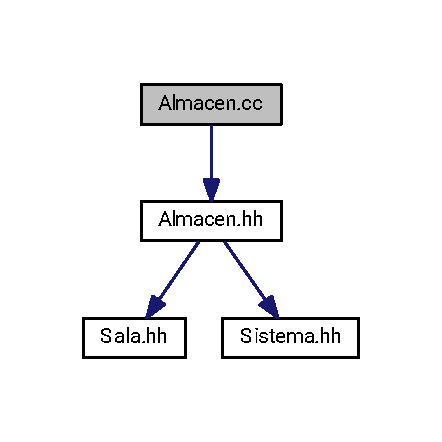
\includegraphics[width=212pt]{_almacen_8cc__incl}
\end{center}
\end{figure}


\subsection{Descripción detallada}
Código de la clase \hyperlink{class_almacen}{Almacen}. 


\hypertarget{_almacen_8hh}{}\section{Referencia del Archivo Almacen.\+hh}
\label{_almacen_8hh}\index{Almacen.\+hh@{Almacen.\+hh}}


Especificación de la clase \hyperlink{class_almacen}{Almacen}.  


Dependencia gráfica adjunta para Almacen.\+hh\+:
\nopagebreak
\begin{figure}[H]
\begin{center}
\leavevmode
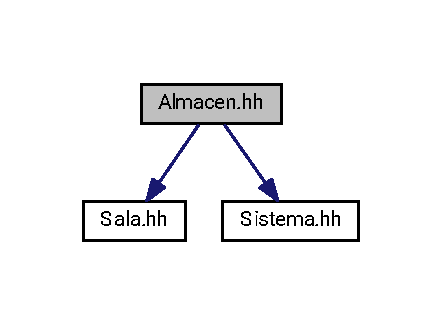
\includegraphics[width=212pt]{_almacen_8hh__incl}
\end{center}
\end{figure}
\subsection*{Clases}
\begin{DoxyCompactItemize}
\item 
class \hyperlink{class_almacen}{Almacen}
\begin{DoxyCompactList}\small\item\em Representa un almacén. \end{DoxyCompactList}\end{DoxyCompactItemize}


\subsection{Descripción detallada}
Especificación de la clase \hyperlink{class_almacen}{Almacen}. 


\hypertarget{program_8cc}{}\section{Referencia del Archivo program.\+cc}
\label{program_8cc}\index{program.\+cc@{program.\+cc}}


Programa principal para el ejercicio {\itshape Tree\+K\+EA}  


Dependencia gráfica adjunta para program.\+cc\+:
\nopagebreak
\begin{figure}[H]
\begin{center}
\leavevmode
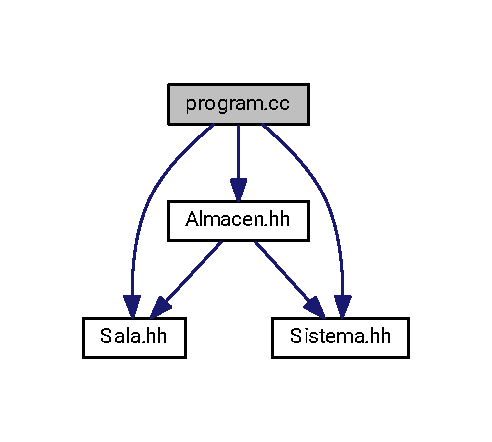
\includegraphics[width=236pt]{program_8cc__incl}
\end{center}
\end{figure}
\subsection*{Funciones}
\begin{DoxyCompactItemize}
\item 
int \hyperlink{program_8cc_ae66f6b31b5ad750f1fe042a706a4e3d4}{main} ()
\begin{DoxyCompactList}\small\item\em Programa principal para el ejercicio {\itshape Tree\+K\+EA} \end{DoxyCompactList}\end{DoxyCompactItemize}


\subsection{Descripción detallada}
Programa principal para el ejercicio {\itshape Tree\+K\+EA} 



\subsection{Documentación de las funciones}
\index{program.\+cc@{program.\+cc}!main@{main}}
\index{main@{main}!program.\+cc@{program.\+cc}}
\subsubsection[{\texorpdfstring{main()}{main()}}]{\setlength{\rightskip}{0pt plus 5cm}int main (
\begin{DoxyParamCaption}
{}
\end{DoxyParamCaption}
)}\hypertarget{program_8cc_ae66f6b31b5ad750f1fe042a706a4e3d4}{}\label{program_8cc_ae66f6b31b5ad750f1fe042a706a4e3d4}


Programa principal para el ejercicio {\itshape Tree\+K\+EA} 



Definición en la línea 27 del archivo program.\+cc.


\begin{DoxyCode}
27            \{
28     \hyperlink{class_almacen}{Almacen} alm;
29     \hyperlink{class_sistema}{Sistema} sist;
30     \textcolor{keywordtype}{int} n, id, f, c, i, j;
31     \textcolor{keywordtype}{string} op, prod;
32     cin >> n;
33     alm.\hyperlink{class_almacen_ae953db6cd573ea3f54e6a02245a25175}{inicializar}(n);
34     cin >> op;
35     \textcolor{keywordflow}{while} (op != \textcolor{stringliteral}{"fin"}) \{
36         \textcolor{keywordflow}{if} (op == \textcolor{stringliteral}{"poner\_prod"}) \{
37             cin >> prod;
38             cout << op << \textcolor{charliteral}{' '} << prod << endl;
39             sist.\hyperlink{class_sistema_af23b15605b8c26c79b1e195eb164a06f}{poner\_prod}(prod);
40         \} \textcolor{keywordflow}{else} \textcolor{keywordflow}{if} (op == \textcolor{stringliteral}{"quitar\_prod"}) \{
41             cin >> prod;
42             cout << op << \textcolor{charliteral}{' '} << prod << endl;
43             sist.\hyperlink{class_sistema_a9e35414af566cf486d09504014a26f40}{quitar\_prod}(prod);
44         \} \textcolor{keywordflow}{else} \textcolor{keywordflow}{if} (op == \textcolor{stringliteral}{"poner\_items"}) \{
45             cin >> \textcolor{keywordtype}{id} >> prod >> n;
46             cout << op << \textcolor{charliteral}{' '} << \textcolor{keywordtype}{id} << \textcolor{charliteral}{' '} << prod << \textcolor{charliteral}{' '} << n << endl;
47             n = alm.\hyperlink{class_almacen_a0285105782dc12b843cbdad492887956}{poner\_items}(\textcolor{keywordtype}{id}, prod, n, sist);
48             \textcolor{keywordflow}{if} (n != -1) cout << \textcolor{stringliteral}{"  "} << n << endl;
49         \} \textcolor{keywordflow}{else} \textcolor{keywordflow}{if} (op == \textcolor{stringliteral}{"quitar\_items"}) \{
50             cin >> \textcolor{keywordtype}{id} >> prod >> n;
51             cout << op << \textcolor{charliteral}{' '} << \textcolor{keywordtype}{id} << \textcolor{charliteral}{' '} << prod << \textcolor{charliteral}{' '} << n << endl;
52             n = alm.\hyperlink{class_almacen_a2ed6c0f1a88f8ba8d2ad2268640a890f}{quitar\_items}(\textcolor{keywordtype}{id}, prod, n, sist);
53             \textcolor{keywordflow}{if} (n != -1) cout << \textcolor{stringliteral}{"  "} << n << endl;
54         \} \textcolor{keywordflow}{else} \textcolor{keywordflow}{if} (op == \textcolor{stringliteral}{"distribuir"}) \{
55             cin >> prod >> n;
56             cout << op << \textcolor{charliteral}{' '} << prod << \textcolor{charliteral}{' '} << n << endl;
57             n = alm.\hyperlink{class_almacen_a257546bb178d1bc7b08443697560281a}{distribuir}(prod, n, sist);
58             \textcolor{keywordflow}{if} (n != -1) cout << \textcolor{stringliteral}{"  "} << n << endl;
59         \} \textcolor{keywordflow}{else} \textcolor{keywordflow}{if} (op == \textcolor{stringliteral}{"compactar"}) \{
60             cin >> id;
61             cout << op << \textcolor{charliteral}{' '} << \textcolor{keywordtype}{id} << endl;
62             alm.\hyperlink{class_almacen_a9b0a893ac5ea4774bd362e297b2c3770}{compactar}(\textcolor{keywordtype}{id});
63         \} \textcolor{keywordflow}{else} \textcolor{keywordflow}{if} (op == \textcolor{stringliteral}{"reorganizar"}) \{
64             cin >> id;
65             cout << op << \textcolor{charliteral}{' '} << \textcolor{keywordtype}{id} << endl;
66             alm.\hyperlink{class_almacen_a9e27219c735096dab9d5d3edc2ae2012}{reorganizar}(\textcolor{keywordtype}{id});
67         \} \textcolor{keywordflow}{else} \textcolor{keywordflow}{if} (op == \textcolor{stringliteral}{"redimensionar"}) \{
68             cin >> \textcolor{keywordtype}{id} >> f >> c;
69             cout << op << \textcolor{charliteral}{' '} << \textcolor{keywordtype}{id} << \textcolor{charliteral}{' '} << f << \textcolor{charliteral}{' '} << c << endl;
70             alm.\hyperlink{class_almacen_a477373756d8671d1acef1c7d84a926a9}{redimensionar}(\textcolor{keywordtype}{id}, f, c);
71         \} \textcolor{keywordflow}{else} \textcolor{keywordflow}{if} (op == \textcolor{stringliteral}{"inventario"}) \{
72             cout << op << endl;
73             sist.\hyperlink{class_sistema_ae56405e21fcc545cb27b0a415752ced4}{inventario}();
74         \} \textcolor{keywordflow}{else} \textcolor{keywordflow}{if} (op == \textcolor{stringliteral}{"escribir"}) \{
75             cin >> id;
76             cout << op << \textcolor{charliteral}{' '} << \textcolor{keywordtype}{id} << endl;
77             alm.\hyperlink{class_almacen_ad9a5ab33dd0c247c5d09496fa7d202f1}{consultar\_sal}(\textcolor{keywordtype}{id}).\hyperlink{class_sala_a31cac453fd5002b715706482b207ac1f}{escribir}();
78         \} \textcolor{keywordflow}{else} \textcolor{keywordflow}{if} (op == \textcolor{stringliteral}{"consultar\_pos"}) \{
79             cin >> \textcolor{keywordtype}{id} >> i >> j;
80             cout << op << \textcolor{charliteral}{' '} << \textcolor{keywordtype}{id} << \textcolor{charliteral}{' '} << i << \textcolor{charliteral}{' '} << j << endl;
81             prod = alm.\hyperlink{class_almacen_ad9a5ab33dd0c247c5d09496fa7d202f1}{consultar\_sal}(\textcolor{keywordtype}{id}).\hyperlink{class_sala_a7a162d097c0f7e295cc17ceb286930b2}{consultar\_pos}(i, j);
82             cout << \textcolor{stringliteral}{"  "} << prod << endl;
83         \} \textcolor{keywordflow}{else} \textcolor{keywordflow}{if} (op == \textcolor{stringliteral}{"consultar\_prod"}) \{
84             cin >> prod;
85             cout << op << \textcolor{charliteral}{' '} << prod << endl;
86             n = sist.\hyperlink{class_sistema_a6e61a7675d9d4c9f5fed403bd29ea021}{consultar\_prod}(prod);
87             \textcolor{keywordflow}{if} (n != -1) cout << \textcolor{stringliteral}{"  "} << n << endl;
88         \}
89         cin >> op;
90     \}
91     cout << op << endl;
92 \}
\end{DoxyCode}

\hypertarget{_sala_8cc}{}\section{Referencia del Archivo Sala.\+cc}
\label{_sala_8cc}\index{Sala.\+cc@{Sala.\+cc}}


Código de la clase \hyperlink{class_sala}{Sala}.  


Dependencia gráfica adjunta para Sala.\+cc\+:
\nopagebreak
\begin{figure}[H]
\begin{center}
\leavevmode
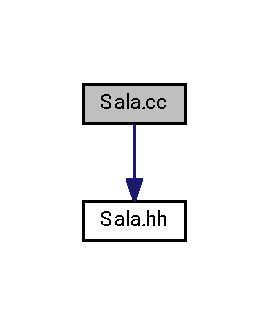
\includegraphics[width=129pt]{_sala_8cc__incl}
\end{center}
\end{figure}


\subsection{Descripción detallada}
Código de la clase \hyperlink{class_sala}{Sala}. 


\hypertarget{_sala_8hh}{}\section{Referencia del Archivo Sala.\+hh}
\label{_sala_8hh}\index{Sala.\+hh@{Sala.\+hh}}


Especificación de la clase \hyperlink{class_sala}{Sala}.  


\subsection*{Clases}
\begin{DoxyCompactItemize}
\item 
class \hyperlink{class_sala}{Sala}
\begin{DoxyCompactList}\small\item\em Representa una sala. \end{DoxyCompactList}\end{DoxyCompactItemize}


\subsection{Descripción detallada}
Especificación de la clase \hyperlink{class_sala}{Sala}. 


\hypertarget{_sistema_8cc}{}\section{Referencia del Archivo Sistema.\+cc}
\label{_sistema_8cc}\index{Sistema.\+cc@{Sistema.\+cc}}


Código de la clase \hyperlink{class_sistema}{Sistema}.  


Dependencia gráfica adjunta para Sistema.\+cc\+:
\nopagebreak
\begin{figure}[H]
\begin{center}
\leavevmode
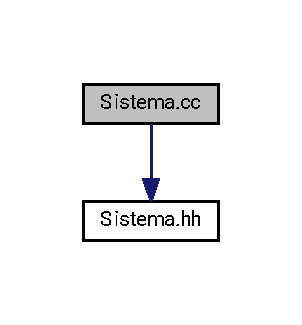
\includegraphics[width=145pt]{_sistema_8cc__incl}
\end{center}
\end{figure}


\subsection{Descripción detallada}
Código de la clase \hyperlink{class_sistema}{Sistema}. 


\hypertarget{_sistema_8hh}{}\section{Referencia del Archivo Sistema.\+hh}
\label{_sistema_8hh}\index{Sistema.\+hh@{Sistema.\+hh}}


Especificación de la clase \hyperlink{class_sistema}{Sistema}.  


\subsection*{Clases}
\begin{DoxyCompactItemize}
\item 
class \hyperlink{class_sistema}{Sistema}
\begin{DoxyCompactList}\small\item\em Representa un sistema. \end{DoxyCompactList}\end{DoxyCompactItemize}


\subsection{Descripción detallada}
Especificación de la clase \hyperlink{class_sistema}{Sistema}. 


%--- End generated contents ---

% Index
\backmatter
\newpage
\phantomsection
\clearemptydoublepage
\addcontentsline{toc}{chapter}{Índice}
\printindex

\end{document}
